\section{\textbf{Introduction}}\label{sec:1}
	DC motors are commonly used in robotics due to it's reduced size, light weight and easy velocity control \todo{add ref}, avoiding the use of rectifiers or power inverters. In order to change the orientation of a DC motor, for instance, only the direction of the applied voltage needs to change.

	H bridges (see Figure~\ref{fig:bridge}) are simple electronic circuits used to enable a voltage to be applied across a motor in either direction. Despite it's simplicity H bridges might be used to accomplish more challenging tasks, such as stabilizing distributed energy sources \todo{add ref} and improving power quality in electric vehicles \todo{add ref}.

\begin{figure*}[t]
\centering
% \begin{subfigure}[b]{0.4\textwidth}
	\centering%
	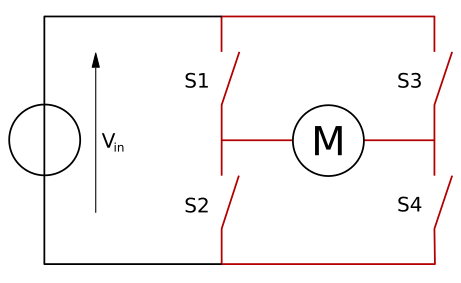
\includegraphics[height=.25\textwidth]{img/H_bridge.png}
	\caption{H Bridge figure borrowed from wikipedia~\cite{WIKI}.}\label{fig:bridge}%
% \end{subfigure}\hfill
\end{figure*}

\begin{figure}[htp!]
\begin{center}
\begin{circuitikz} %\label{sec:1}
    \draw (2,0) node[npn](q1) at (2,0){}
    (q1.E) node[npn](q4) at (2,-1.55){}
    (q1.E) -- (q4.C);
    \draw (-0.55,0) to[R] (q1.B){};
    \draw (-0.55,-1.55) to[R] (q4.B){};
    \draw (5,0) node[npn,xscale=-1](q3) at (4,0){}
    (q3.E) node[npn,xscale=-1](q2) at (4,-1.55){}
    (q3.E) -- (q2.C)
    (q1.C) -- (q3.C)
    (q4.E) -- (q2.E);
    \draw (3,-2.55) node[ground](gnd){}
    (q2.E) |- (gnd);
    \draw (q3.B)  to[R] (6,0);
    \draw (q2.B) to[R] (6,-1.55);
    % \draw (q1.E) node[elmech]{M}) (q3.E);
    \draw (-0.55,0) -- (-1.0,0) node[circ]{} -- (-1.0,-4) -- (7,-4) -- (7,-1.55) -- (6,-1.55);
    \draw (-0.55,-1.55) -- (-0.80,-1.55) -- (-0.8,-3.5) --(6.5,-3.5) -- (6.5,0) node[circ]{} -- (6,0);
    \draw (3,2) node[spdt,xscale=-1] (s1){}
    (s1.in) |- node[circ]{} (q1.C)
    (s1.out 1) |- (3.5,2.5) |- (7,2.5) |- (6,0)
    (s1.out 2) |- (-1,1.685) |- (-1,0);
    \draw (q1.E) to[sV, color=white, name=M1] (q3.E);
    \mymotor{M1}{0}
    \draw (q2.E) node[circ]{} |- (7.5,-2.31) to[battery] (7.5,1) |- (4,1) |- node[circ]{} (q3.C);
    % \draw (q1.C) --++(0,0.5) node[vcc]{+4.5\,\textnormal{V}};
    % \mymotor{M}{0}
    % \draw (q1.B) -- to[R=100<\ohm>]{};
    % \draw (0,0) node[npn](npn) at (0,0){};
\end{circuitikz}
\caption{H Bridge}\label{fig:schem}%
\end{center}
\end{figure}

